\subsection{The Photon}

What led to the development of quantum mechanics was spirited debate about the true nature of light.
Newton was one of the first to throw his hat into the ring; in 1672 he decided to build upon the corpuscular theory coined by Descartes, arguing that light was made up of discrete particles just like everything else.
Problem was, that around the same time Robert Hooke and Christian Huygens performed experiments  that led them to believe light was in fact not a stream of particles but rather a wave.
This wave view of light did a much better job of explaining how light refracted compared to Newtons model.

The position of people beliving that light was in fact a wave, not particles got a lot stronger in 1801 thanks to double slit experiments by Thomas Young.
This was an experiment where there were two slits cut into a screen and light was then shone through it being visible on another screen once it had made it past the slits.
If light was indeed made up of particles, the expectation was that we would see essentially 2 bright spots on the final screenthat corresponded to the two slits.
Instead, what we got was an interference pattern that iss typical of waves.

\begin{figure}[H]
  % https://en.wikipedia.org/wiki/Double-slit_experiment#/media/File:Double-slit.svg
  \centering
  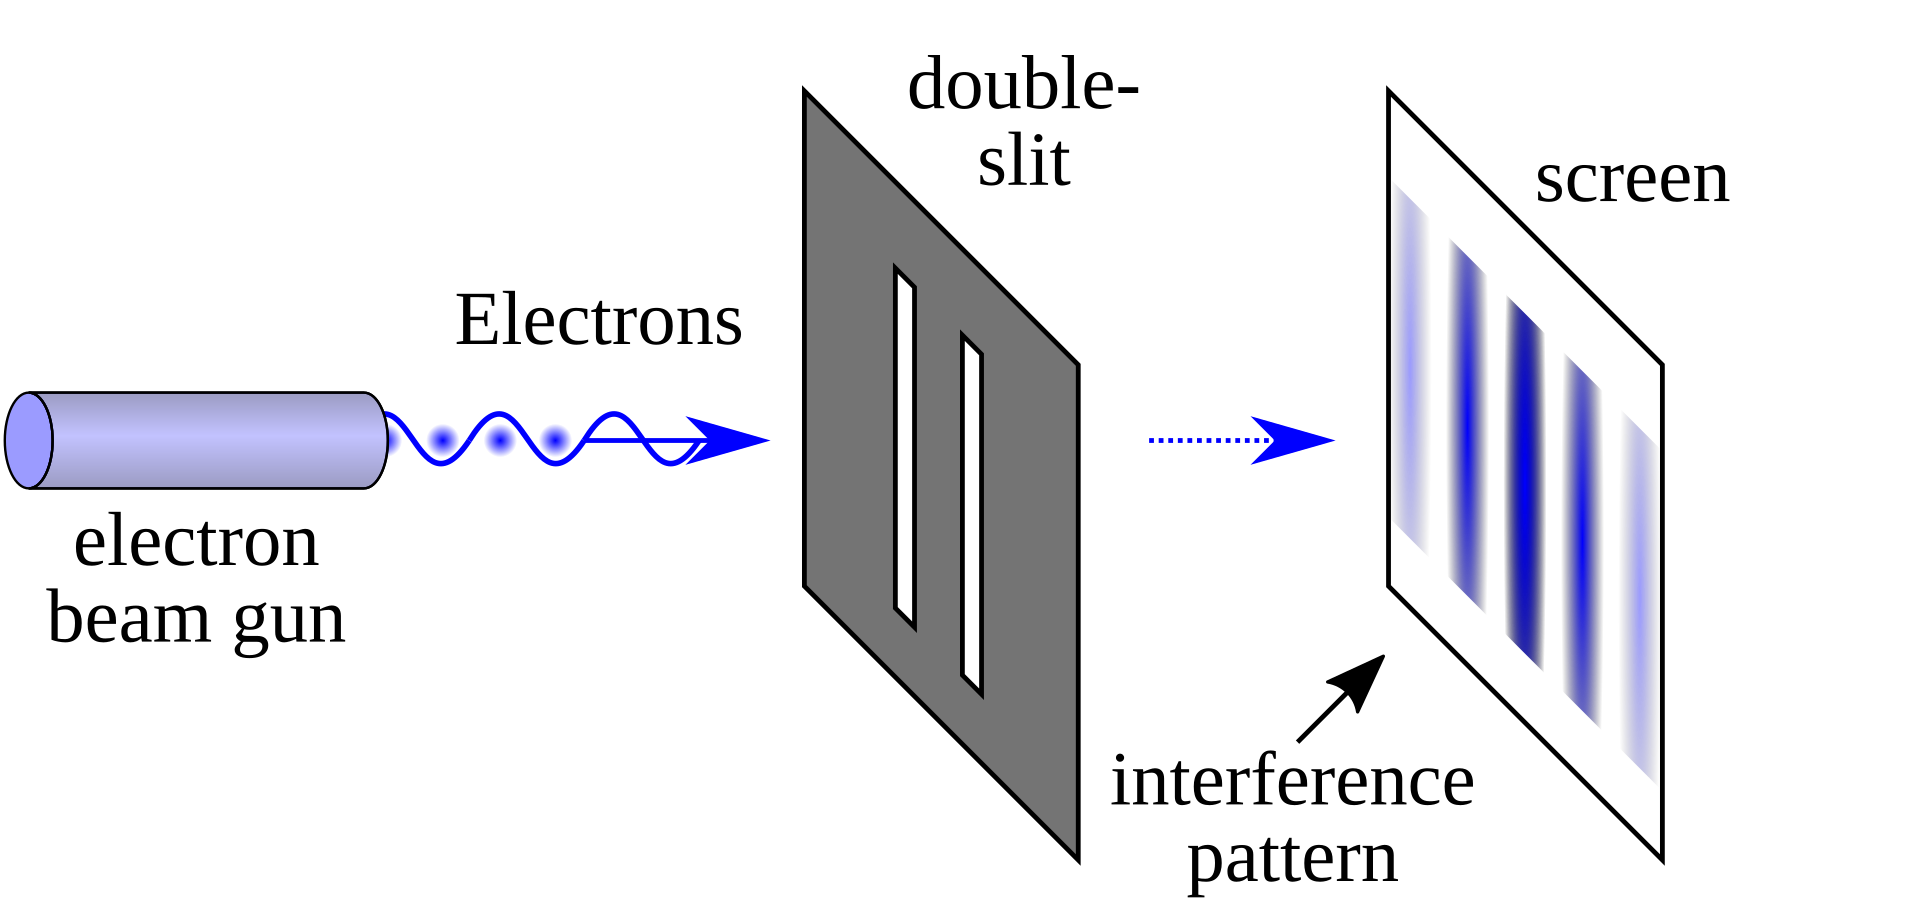
\includegraphics[width=130mm]{figures/doubleSlit.png}
  \caption{Double Slit Experiment}
  \label{doubleSlit}
\end{figure}

At this point, the world is pretty much in the wave camp for the purposes of modelling light, but the idea that light is made of particles was about to be revived from the dead by none other than Max Planck.
He was trying to solve the problem of black body radiation; namely, that the energy carried by electromagnetic waves is emitted and absorbed in discrete quantities.
His solution was to  come up with the idea of discrete quanta rather than a continously emmisive spectrum.
He did this through the creation of the what we call the Planck constant today ($h$), a proportionality constant  that he called  the quantum of action.

This was fundamentally the introduction of quantum mechanics.  a quite contentious idea at the time, highlighted by the following quote from Bohr.

quantum theory cannot possibly have understood it.

\begin{flushright}--- Neils Bohr\end{flushright}

Despite being frought in debate, the idea of quantum mechanics simply would not go away.
Einstein would go on to build on the Planck's ideas and proposed that light was made up of discrete packets of energy that he called photons.
He developed the Planck-Einstein Relationship, connecting  energy and the frequency of light.

\begin{align}
  E = h \nu
\end{align}

Where $E$ stands for energy, $h$ for thePlanck constant and $\nu$ for the frequency of the photon.

% Could you please check if the equation is correct, I'm not totally sure about the \nu

This equation was to explain the results that Einstein had gotten from his experiments regarding the photoelectric effect.
In 1914, Robert A. Millikan went on to confirm Einstein's idea by doing  a highly accurate measurement of Plank's Constant  using the photoelectric effect.
Photons would go on to be included in the list of particles we deal with in the standard model today.

This new evidence went in the face of the wave nature of light which had been longstanding.
It seemed like  there were phenomena that could be explained by thinking of light as a wave and other phenomena that could be understood if we looked at light as a particle.

